%!TEX root = PhD_Thesis.tex
\chapter{Introduction}

%%%%%%%%%%%%%%%%%%%%%%%%%%%%%%%%%%%%%%%%%%%%%%%%%%%%%%%%%%%%%%%%%%%%%%%%%%%%%%%%%%%%%%%%%%%%%%%%%%%%======================================================================
\section{Motivation}
%======================================================================
%%%%%%%%%%%%%%%%%%%%%%%%%%%%%%%%%%%%%%%%%%%%%%%%%%%%%%%%%%%%%%%%%%%%%%%%%%%%%%%%%%%%%%%%%%%%%%%%%%%
\subsection{Percutaneous Interventions}
Needles are slim metal tubes with sharpened tips that puncture the skin and other intervening tissues to allow access to internal anatomy. Needles are ubiquitous tools in modern medicine. They are applied in a range of form factors by clinicians in many specialties to inject drugs, drain fluids, remove tissue samples for testing, or deposit implants. Interventional radiology is a medical specialty that uses instruments inserted through needles under medical image guidance to treat disease. Such percutaneous interventions are increasingly favored as alternatives to surgery, because they result in less trauma to the patient, and thus reduce the risk of complications and patient recovery time. 

\subsection{Liver Cancer}
The liver is a glandular organ that sits in the right side of the abdomen in humans. It weighs approximately 1.2~kg to 1.5~kg and is approximately 14~cm long on average in adults~\cite{Wolf1990,Kratzer2003}. Structurally, the liver is divided into two lobes, as shown in Fig.~\ref{fig:Ch1LiverAnatomy}. Its primary function is to filter blood coming from the digestive tract before it passes on to the rest of the body. 

\begin{figure}[!h]
\centering
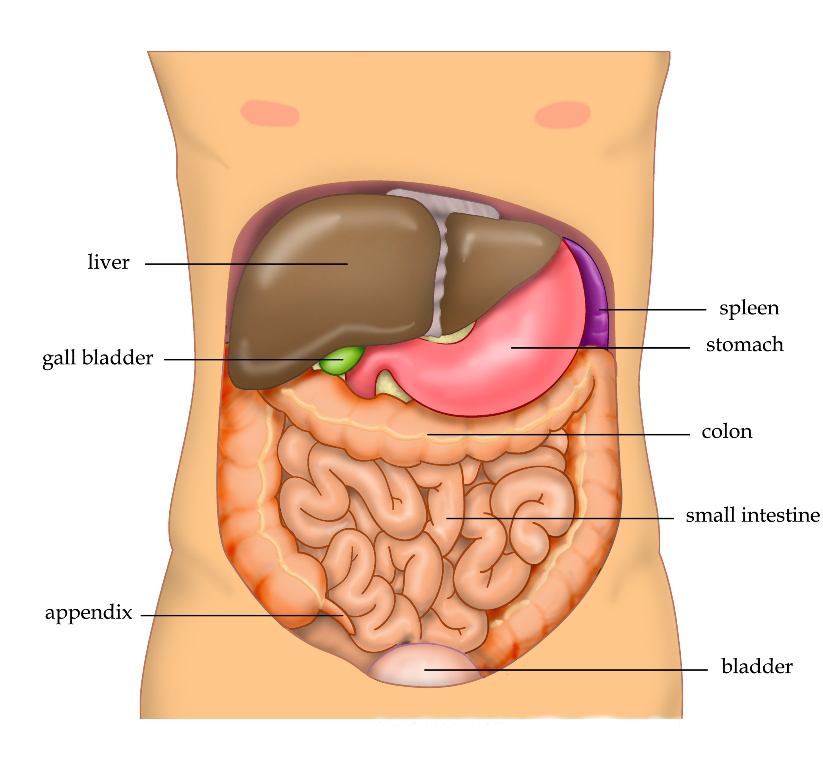
\includegraphics[width = 0.75\columnwidth]{./Images/Chapter1/liverIllustration.jpg}%
\caption{Anatomy of the human liver. Image courtesy WebMD LLC.}
\label{fig:Ch1LiverAnatomy}
\end{figure}    

Liver cancer is a significant health concern in the United States. Liver cancer can be subdivided into primary liver cancer, where the disease originates in the cells of the liver, and secondary liver cancer, where the cancer originates in other organs and metastasizes to the liver. Approximately 35,660 new cases of primary liver cancer will be diagnosed in the United States in 2015, and approximately 24,550 people will die of these cancers~\cite{AmericanCancer2015}. Secondary liver cancers occur more frequently. Common types of cancers such as breast, lung, and colon cancer all metastasize to the liver. For example, a quarter of the approximately 130,000 patients diagnosed with colorectal cancer each year in the United States will develop liver metastases~\cite{Ananthakrishnan2006,CDC2015,Haddad2011}. Liver cancer is an even more significant health concern in other parts of the world. Liver cancer is the most common type of cancer in many countries in sub-Saharan Africa and Southeast Asia. More than 700,000 people are diagnosed with this cancer each year throughout the world, with more than 600,000 deaths annually~\cite{AmericanCancer2015}.

\subsection{Treatment of Liver Tumors}
While transplantation and resection offer the best long-term survival in select patients, they are not possible in at least 70 percent of patients due to tumor size, type, or location; inadequate liver reserve; or other comorbidities. Additionally, tumor recurrence in 5 years exceeds 70 percent in patients who undergo surgical resection of hepatocellular carcinoma (HCC) [14]. 



Percutaneous radiofrequency ablation (RFA) is a less invasive option to treat patients with cancer in the liver and could become the preferred method if success rates improve. RFA kills tumors in situ by depositing a high-frequency alternating current in the tissue, which causes ionic agitation and frictional heating; the heat leads to thermal damage of tissue around ablation probes. While the ability to treat liver tumors with minimal loss of functional liver tissue and minimal bleeding risk is highly desirable, current technical limitations have precluded broader adoption of RFA as a means of eradicating liver tumors [26]. Tumors in some portions of the liver cannot be accessed because the straight paths currently taken by RFA electrodes would traverse vasculature, lung, or other sensitive structures. Large tumors require multiple electrode insertions, and the increased bleeding risk with each liver capsule puncture can be too great in patients with advanced liver disease or severe comorbidities. Successful treatment of larger tumors is highly dependent on the clinician’s ability to accurately localize the electrode tip over multiple passes [22]. The high local recurrence rate after percutaneous RFA suggests that, even in experienced hands, it is difficult to accurately ablate the entirety of a tumor due to failure to achieve appropriate overlap of ablation zones [38,66]. [Only 12 percent of HCC patients and a smaller fraction of patients with metastatic tumors are currently treated with RFA or other forms of ablation [44]; this could at least double with increased safety and accuracy of RFA [26]. From incidence/treatment statistics, we estimate that this would enable an additional 5,000 cases of liver cancer to be treated with RFA each year.]

\subsection{Robotic Needle Steering}

%%%%%%%%%%%%%%%%%%%%%%%%%%%%%%%%%%%%%%%%%%%%%%%%%%%%%%%%%%%%%%%%%%%%%%%%%%%%%%%%%%%%%%%%%%%%%%%%%%%%======================================================================
\section{Contributions}
%======================================================================
%%%%%%%%%%%%%%%%%%%%%%%%%%%%%%%%%%%%%%%%%%%%%%%%%%%%%%%%%%%%%%%%%%%%%%%%%%%%%%%%%%%%%%%%%%%%%%%%%%%
We briefly summarize the major contributions of this dissertation as follows:
\begin{itemize}
\item We did some stuff.
\item We did some more stuff.
\end{itemize}


%%%%%%%%%%%%%%%%%%%%%%%%%%%%%%%%%%%%%%%%%%%%%%%%%%%%%%%%%%%%%%%%%%%%%%%%%%%%%%%%%%%%%%%%%%%%%%%%%%%%======================================================================
\section{Prior Work}
%======================================================================
%%%%%%%%%%%%%%%%%%%%%%%%%%%%%%%%%%%%%%%%%%%%%%%%%%%%%%%%%%%%%%%%%%%%%%%%%%%%%%%%%%%%%%%%%%%%%%%%%%%

\subsection{Techniques for Needle Steering}


\subsection{Automatic Segmentation of Needles from Ultrasound Data}
\cite{Adebar2013}
\cite{Adebar2015}

\subsection{Control Approaches for Robotic Needle Steering}


%%%%%%%%%%%%%%%%%%%%%%%%%%%%%%%%%%%%%%%%%%%%%%%%%%%%%%%%%%%%%%%%%%%%%%%%%%%%%%%%%%%%%%%%%%%%%%%%%%%%======================================================================
\section{Dissertation Overview}
%======================================================================
%%%%%%%%%%%%%%%%%%%%%%%%%%%%%%%%%%%%%%%%%%%%%%%%%%%%%%%%%%%%%%%%%%%%%%%%%%%%%%%%%%%%%%%%%%%%%%%%%%%

This thesis consists of six chapters. In chapter 1, which is this introduction, we presented the motivation for our research of using tactile feedback for sensory substitution and augmentation of force feedback. We also presented prior work on the various types of tactile feedback devices and prior work on providing interaction force information in robot-assisted minimally invasive surgery.

Chapter 2 describes doppler imaging...

Chapter 3 describes needles...

Chapter 4 describes teleoperation...

Chapter 5 summarizes the results of this research, reviews the contribution made in this dissertation, and provides suggestions for future work.